\let\negmedspace\undefined
\let\negthickspace\undefined
\documentclass[journal,12pt,twocolumn]{IEEEtran}
\usepackage{cite}
\usepackage{amsmath,enumitem,amssymb,amsfonts,amsthm}
\usepackage{algorithmic}
\usepackage{graphicx}
\usepackage{float}
\usepackage{textcomp}
\usepackage{xcolor}
\usepackage{caption}
\usepackage{txfonts}
\usepackage{listings}
\usepackage{enumitem}
\usepackage{mathtools}
\usepackage{gensymb}
\usepackage{comment}
\usepackage[breaklinks=true]{hyperref}
\usepackage{tkz-euclide} 
\usepackage{listings}
\usepackage{tabularx}
\usepackage{gvv}                                        
\def\inputGnumericTable{}                                 
\usepackage[latin1]{inputenc}                              
\usepackage{color}                                            
\usepackage{array}                                            
\usepackage{longtable}                                       
\usepackage{calc}                                             
\usepackage{multirow}                                         
\usepackage{hhline}                                           
\usepackage{ifthen}                                        
\usepackage{lscape}
\newtheorem{theorem}{Theorem}[section]
\newtheorem{problem}{Problem}
\newtheorem{proposition}{Proposition}[section]
\newtheorem{lemma}{Lemma}[section]
\newtheorem{corollary}[theorem]{Corollary}
\newtheorem{example}{Example}[section]
\newtheorem{definition}[problem]{Definition}
\newcommand{\BEQA}{\begin{eqnarray}}
\newcommand{\EEQA}{\end{eqnarray}}
\newcommand{\define}{\stackrel{\triangle}{=}}
\theoremstyle{remark}
\newtheorem{rem}{Remark}
\usepackage{float}
\usepackage{adjustbox}
\usepackage{siunitx}
\usepackage[siunitx]{circuitikz}
\parindent 0px


\begin{document}
\bibliographystyle{IEEEtran}
\vspace{3cm}


\title{GATE: 51.2023}
\author{EE22BTECH11005- Ambati Krishna Kaustubh$^{*}$% <-this % stops a space
}

\maketitle
\newpage
\bigskip

\textbf{Question:}For the circuit shown,if $i=\sin 1000t$, the instantaneous value of the Thevenin's voltage(in volts) across the terminals a anb b at time t=5ms is\\[2pt]

\begin{circuitikz}[american voltages,american currents]
    % Draw the circuit components
    \draw (0,0) -- (2,0);
    \draw (2,2) to [resistor,l=$10\Omega$] (2,4);
    \draw (2,4) -- (0,4);
    \draw (2,0) to [capacitor,l=$-j10\Omega$,*-*,i_=$i_x$] (2,2);
    \draw (2,0) -- (5,0);
    \draw (5,0) to[inductor,l=$j10\Omega$] (5,2);
    \draw (5,2) to [resistor,l=$10\Omega$] (5,4);
  \draw (5,4) to [cV,l^=$4i_x$,invert] (2,4);
  \draw (5,4) -- (6,4);
  \draw (6,4) to[I,l=$\sin 1000t$,invert] (6,0);
  \draw (6,0) -- (5,0);
   \node[circle,fill=black,inner sep=1.5pt,label=above:a] at (0,0) {};
    \node[circle,fill=black,inner sep=1.5pt,label=above:b] at (0,4) {};
    \end{circuitikz}\\[4pt]

\solution By source transforming the given circuit we get\\[2pt]
\begin{circuitikz}[american voltages,american currents]
    % Draw the circuit components
    \draw (0,0) -- (2,0);
    \draw (2,4) to [resistor,l=$10\Omega$,*-*,i_=$i_x$](2,2);
    \draw (2,4) -- (0,4);
    \draw (2,2) to [capacitor,l=$-j10\Omega$] (2,0);
    \draw (2,0) -- (5,0);
    \draw (5,0) to[V,l=$(10+10j)\sin1000t$,invert] (5,1);
    \draw (5,1) to[inductor,l=$j10\Omega$] (5,2);
    \draw (5,2) to [resistor,l=$10\Omega$] (5,4);
  \draw (5,4) to [cV,l^=$4i_x$,invert] (2,4);
   \node[circle,fill=black,inner sep=1.5pt,label=above:a] at (0,0) {};
    \node[circle,fill=black,inner sep=1.5pt,label=above:b] at (0,4) {};
    \end{circuitikz} \\[2pt]

Solving using sinusoidal steady state analysis,
\begin{circuitikz}[american]
    % Draw the circuit components
    \draw (0,0) -- (2,0);
    \draw (2,4) to [european resistor,l=$10\Omega$,*-*,i_=$I_x$](2,2);
    \draw (2,4) -- (0,4);
    \draw (2,2) to [european resistor,l=$X_c(\frac{1}{j\omega C})$] (2,0);
    \draw (2,0) -- (5,0);
    \draw (5,0) to[V,l=$10\angle 45^\circ$,invert] (5,1);
    \draw (5,1) to[european resistor,l=$X_L(j\omega L)$] (5,2);
    \draw (5,2) to [european resistor,l=$10\Omega$] (5,4);
  \draw (5,4) to [cV,l^=$4I_x$,invert] (2,4);
   \node[circle,fill=black,inner sep=1.5pt,label=above:a] at (0,0) {};
    \node[circle,fill=black,inner sep=1.5pt,label=above:b] at (0,4) {};
    \end{circuitikz} 

Applying KVL we get,
\begin{align}
    10 \angle 45^\circ-(j\omega L)I_x-10I_x+4I_x-10I_x-(\frac{1}{j\omega C})I_x=0
\end{align}
\begin{align}
    I_x=\frac{10 \angle 45^\circ}{16+j\omega L+\frac{1}{j\omega C}}
\end{align}
\begin{align}
    V_{ab}=I_x(10+\frac{1}{j\omega C})
\end{align}
\begin{align}
    V_{ab}=\frac{10\angle 45^\circ(10j\omega C+1)}{16j\omega C-\omega^2LC+1}
    \end{align}
    From the question we can observe that,
    \begin{align}
        \frac{1}{\omega C}=\omega L
    \end{align}
    \begin{align}
        \omega^2LC=1 \label{eq:equation}
    \end{align}
Substituting $\ref{eq:equation}$ and values of $\omega C$ and $\omega L$ 
\begin{align}
    V_{ab}=12.5\angle 0^\circ
\end{align}
\begin{align}
    V_{ab}=12.5\sin{1000t}
\end{align}

\begin{figure}[H]
  \centering
  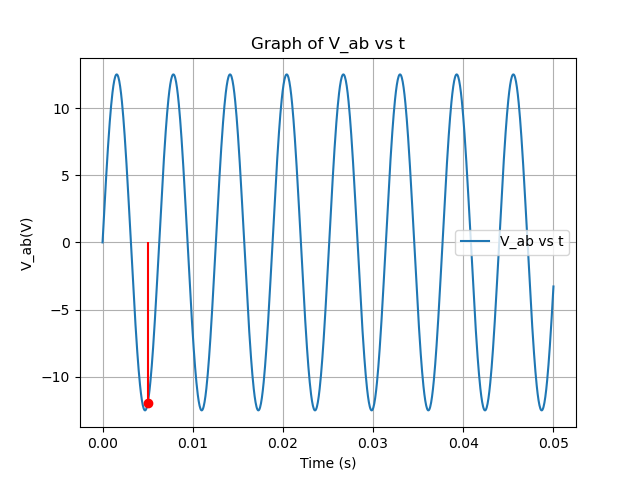
\includegraphics[width=0.5\textwidth]{figs/gate.png} % Include your image file here
  \label{fig:example}
\end{figure}

\end{document}

